\chapter{\IfLanguageName{dutch}{proof-of-concept}{proof-of-concept}}%
\label{ch:proof-of-concept}
\section{Inleiding}
In dit hoofdstuk bespreken we de implementatie van het proof-of-concept. We zullen elke fase van het proces in detail bespreken en de implementatie van de bijbehorende componenten toelichten. Hierbij zullen we ook de uitkomsten van elke fase beschrijven en hoe deze kunnen gebruikt worden in de volgende fase. \\

\section{Webscraper}
\subsection{Algemene Eisen}
Binnen de algemene eisen zal de webscraper voldoen aan de ethische aspecten \ref{subsection:scraper-ethische-aspecten} die zijn beschreven in de state of the art van dit onderzoek. Dit betekent dat de scraper de regels en richtlijnen van de gescrapte websites zal respecteren en zich zal houden aan eventuele beperkingen zoals vermeld in het robots.txt-bestand. Hierdoor wordt ervoor gezorgd dat de scrapingactiviteiten op een ethisch verantwoorde manier worden uitgevoerd. \\

Daarnaast zal de webscraper in staat zijn om verschillende websites te scrapen, met de focus op het verzamelen van de frontpage-inhoud. Specifiek zal de scraper de eerste 20 items van de frontpage van elke website verzamelen. \\

De webscraper zal twee bekende nieuwsbronnen scrapen, namelijk HLN en DeMorgen.

\subsection{Verkenning}
Alvorens we de webscraper kunnen implementeren, is het nodig om de DOM van beide websites te bekijken en een patroon hierin te herkennen. \\
\subsubsection{HLN}
Op de startpagina van HLN kunnen we zien (figuur \ref{fig:hln_frontpage}) dat elk nieuwsartikel zich bevindt binnen een article-tag bevindt. De eerste subtag is een a-tag met hierin de href naar het artikel. \\ Deze href zal belangrijk zijn om de datum te valideren en de titel te extraheren. We moeten deze dus opslaan. 

\begin{center}
    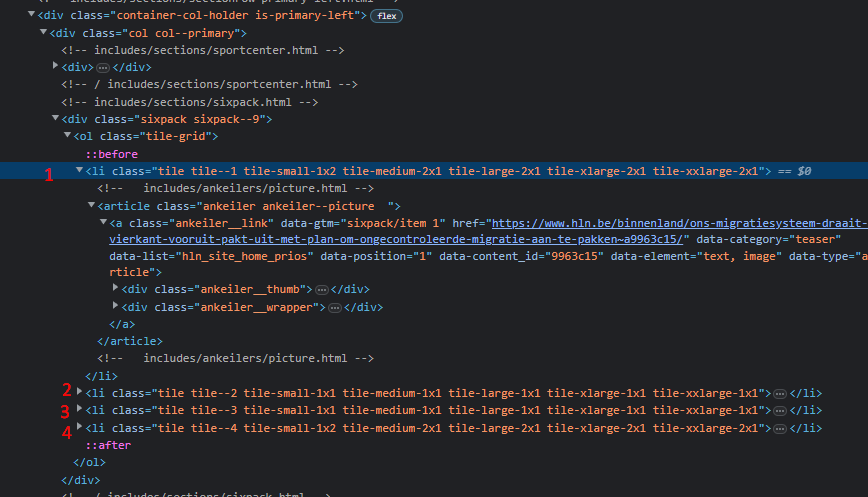
\includegraphics[width = 6in]{hln_frontpage2.png}
    \captionof{figure}{DOM van de startpagina van HLN met aangeduide nieuwsartikels.}
    \label{fig:hln_frontpage}
\end{center}

Als we vervolgens gaan kijken naar de DOM van een artikel, zien we dat de titel weergegeven wordt binnen een header-tag met als class 'article\_\_header' deze titel heeft als class 'article\_\_title'. De datum wordt weergegeven binnen een time-tag met datetime als value en class 'article\_\_time'. De datum is ook opgemaakt in een bepaald formaat, dd-mm-yy, hh:mm. Deze gegevens zijn essentieel voor de scraper. In figuur \ref{fig:hln_article} vind je dit terug. \\

\begin{center}
    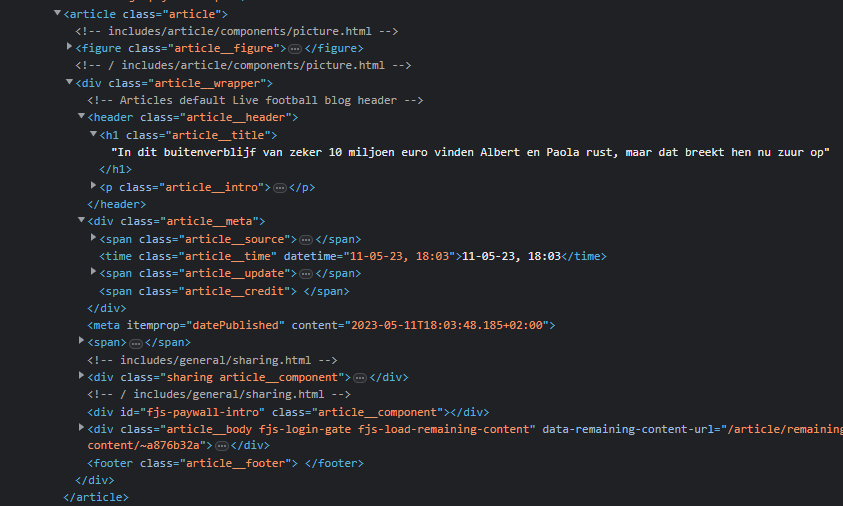
\includegraphics[width = 6in]{hln_article1.png}
    \captionof{figure}{DOM van een artikel op HLN met de essentiële elementen gemarkeerd.}
    \label{fig:hln_article}
\end{center}

\subsubsection{De Morgen}
De structuur van de artikels op de startpagina van De Morgen is vergelijkbaar met die van HLN. Zoals te zien is in figuur \ref{fig:demorgen_frontpage}, worden de artikels ook weergegeven binnen een article-tag, alleen is bij de morgen de tweede child de a-tag ten opzichte van HLN.

\begin{center}
    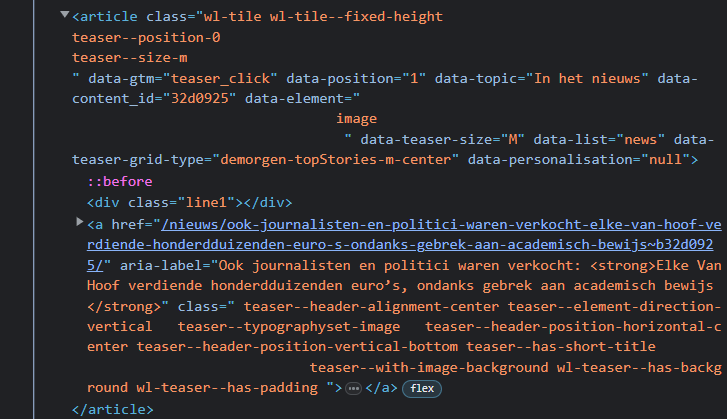
\includegraphics[width = 6in]{demorgen_frontpage2.png}
    \captionof{figure}{DOM van een artikel op De Morgen.}
    \label{fig:demorgen_frontpage}
\end{center}

Bij het doorklikken op een willekeurig artikel zien we dat de DOM vergelijkbaar is, maar niet exact hetzelfde qua structuur. In figuur \ref{fig:demorgen_article} zie je de DOM.

\begin{center}
    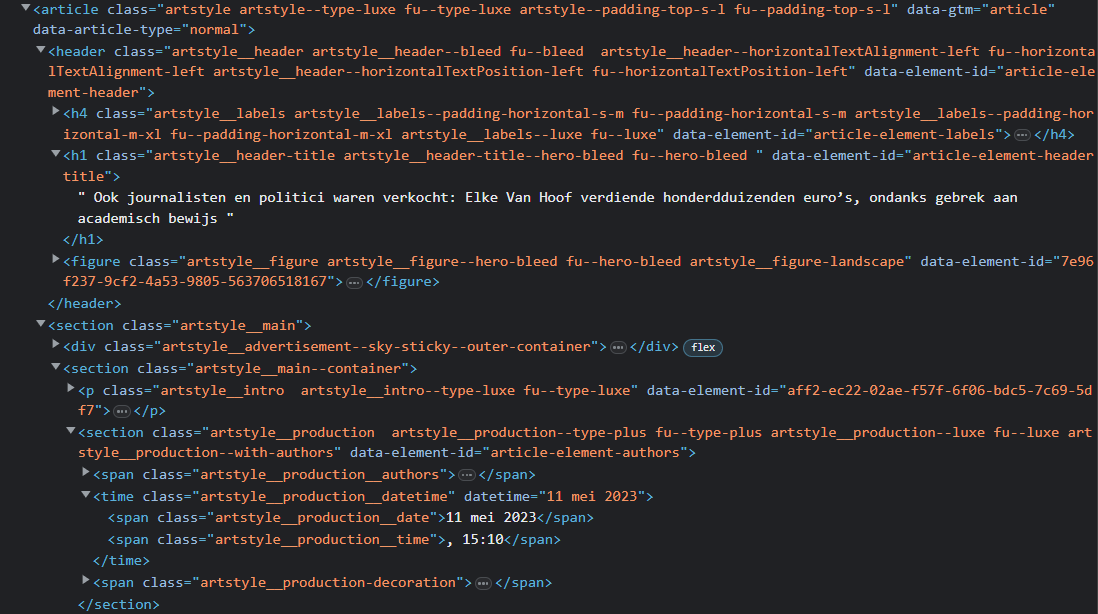
\includegraphics[width = 6in]{demorgen_article.png}
    \captionof{figure}{DOM van een artikel op De Morgen.}
    \label{fig:demorgen_article} 
\end{center}

Nu dat we deze informatie hebben. Kunnen we beginnen aan de implementatie van de scraper. 

\subsection{Implementatie}
\subsubsection{Thread-safe Dictionary}
Om ervoor te zorgen dat de gescrapete data veilig wordt opgeslagen, beginnen we de implementatie met het maken van een thread-safe dictionary.
\begin{pythoncode}{../../../workspace/paper/scraper/util/volatileDictionary.py}
Deze thread-safe dictionary zal de opslag van de gescrapete data beheren en ervoor zorgen dat er geen problemen ontstaan tijdens het wegschrijven van de gescrapete data.
\end{pythoncode}

\subsubsection{Abstracte Thread}
Voordat we de specifieke threads implementeren, maken we eerst een AbstractThread-klasse die de methoden definieert die door de specifieke threads zullen worden gebruikt.

De AbstractThread-klasse bevat het volgende:

\begin{itemize}
    \item \textbf{Constructor}: Initialiseert de gemeenschappelijke eigenschappen die vereist zijn door de specifieke threads.
    \item \textbf{Methoden}: Definieert de gemeenschappelijke methoden die door de specifieke threads zullen worden gebruikt.
\end{itemize}

Laten we de \textbf{constructor} van de AbstractThread-klasse bespreken:

\begin{pythoncode}{../../../workspace/paper/abstractThreadCTR.py}
    In de constructor initialiseren we de gemeenschappelijke eigenschappen die vereist zijn door de specifieke threads. Deze eigenschappen omvatten:
\end{pythoncode}

    \begin{itemize}
        \item \textbf{dict}: De thread-safe dictionary die gebruikmaakt van dependency injection en geïnitialiseerd wordt.
        \item \textbf{limit}: De maximum waarde waarvan de artikels ouder moeten zijn.
        \item \textbf{articles}: De artikels die moeten worden verwerkt.
        \item \textbf{dateformat}: Het formaat van de datum dat wordt weergegeven in de artikelen.
        \item \textbf{title\_tag, title\_class, time\_tag, time\_class}: De HTML klassen waar de relevante gegevens in voorkomt.
        \item \textbf{base\_url}: De URL waarop de scraper moet starten.
        \item \textbf{routes}: De routes waarop de scraper toegestaan is te scrapen, rekening houdend met robots.txt terug te vinden op punt \ref{ch:liter_webscraping}.
        \item \textbf{headers}: De headers die aan de verzoeken worden toegevoegd om toegang te krijgen tot de website.
        \item \textbf{current}: Het momenteel verwerkte artikel.
        \item \textbf{article\_link}: De link van het huidige artikel dat overeenkomt met de opgegeven routes en momenteel wordt gescraped. \\
    \end{itemize}

Daarnaast bevat de AbstractThread-klasse ook verschillende methoden die het scrapen mogelijk maken. Laten we deze methoden bespreken:

\begin{pythoncode}{../../../workspace/paper/abstractThreadONSTART.py}
 Deze methode stuurt een initiële aanvraag naar de base\_url om de eerste 20 artikelen op te halen.
\end{pythoncode}

\begin{pythoncode}{../../../workspace/paper/abstractThreadSTARTSCRAPING.py}
Deze methode voert de on\_start()-methode uit, die de initiële artikelen ophaalt. Vervolgens gaat het door met het scrapen van artikelen zolang er artikelen in de lijst zijn. Elk artikel wordt gecontroleerd met behulp van de should\_scrape\_article()-methode en als het aan de voorwaarden voldoet, wordt het gescraped met behulp van de scrape\_article()-methode.
\end{pythoncode}

\begin{pythoncode}{../../../workspace/paper/abstractThreadSHOULDSCRAPE.py}
Deze methode controleert of de URL van een artikel overeenkomt met een van de opgegeven base\_urls. Als dit het geval is, wordt de article\_link ingesteld en wordt True geretourneerd om aan te geven dat het artikel moet worden gescraped.
\end{pythoncode}

\begin{pythoncode}{../../../workspace/paper/abstractThreadSCRAPE.py}
    Deze methode haalt de inhoud van de article\_link op met behulp van een GET-verzoek en de opgegeven headers. Vervolgens worden de datum en titel geëxtraheerd op basis van de opgegeven HTML-klassen. Als de geëxtraheerde datum vandaag is, wordt de append\_to\_dict()-methode aangeroepen om het artikel op te slaan in de thread-safe dictionary. \\
    
    Na elke request naar een bepaald artikel wordt er een korte sleep geïmplementeerd zodat we niet overdrijven in het aantal request dat we versturen om de server niet te overbelasten zoals besproken in punt \ref{subsection:scraper-ethische-aspecten}.
\end{pythoncode}

De AbstractThread-klasse biedt een basis voor het implementeren van de specifieke threads.

\subsubsection{HLNThread}
    De HLNThread wordt aangemaakt met de volgende code:
    
\begin{pythoncode}{../../../workspace/paper/hlnThread.py}
    De HLNThread wordt geïnitialiseerd met de specifieke eigenschappen die vereist zijn voor het scrapen van artikelen op de HLN-website. Het base\_url is "https://www.hln.be" en de routes zijn ["/buitenland", "/binnenland", "/vtm-nieuws"]. De HTML-klassen voor de titel en de datum worden ook opgegeven.
\end{pythoncode}

\subsubsection{De Morgen Thread}
    De DeMorgenThread wordt aangemaakt met de volgende code:

\begin{pythoncode}{../../../workspace/paper/deMorgenThread.py}
    De DeMorgenThread wordt geïnitialiseerd met de specifieke eigenschappen die vereist zijn voor het scrapen van artikelen op de De Morgen-website. De base\_url is "https://www.demorgen.be" en de routes moeten nog worden toegevoegd, afhankelijk van de specifieke routes op de website van De Morgen doen we dit binnenin de on\_start()-methode om zo steeds de up-to-date routes te hebben. De HTML-klassen voor de titel en de datum worden ook opgegeven.x
\end{pythoncode}

\subsection{Uitkomst}
Om de uitkomst hiervan te testen, maken we een nieuw bestand aan genaamd \_\_main\_\_.py en gebruiken we dit bestand als het startpunt van onze applicatie. Hieronder vind je de inhoud van \_\_main\_\_.py:
\begin{pythoncode}{../../../workspace/paper/scraperMain.py}
In de main functie starten we het scrapingproces door de start\_scraping()-methode aan te roepen. De gescrapete gegevens worden opgeslagen en geprint op de console. \\

De start\_scraping functie initialiseert een VolatileDict object om de gescrapete gegevens op te slaan. Vervolgens maken we instanties van de specifieke threads en voegen we ze toe aan de lijst threads. We gebruiken een ThreadPoolExecutor om de threads parallel uit te voeren en slaan de resultaten op in de futures lijst. \\

Na het voltooien van alle threads halen we de gescrapete gegevens op met behulp van de output\_dict() methode van het VolatileDict object. Deze gegevens worden geretourneerd als het resultaat van de functie. \\

Dit is een basisimplementatie van het startpunt van de applicatie, die in volgende stappen wordt aangepast en uitgebreid.
\end{pythoncode}

Hieronder vindt je het resultaat van Vrijdag 19/05/2023, 20:07u.
\begin{listing}[H]
    \begin{minted}[breaklines]{json}
{
    "https://www.hln.be": [
    "Nederlander (37) overlijdt na ongeval met ontplofte petanquebal tijdens vrijgezellenfeest in Stavelot",
    "EXCLUSIEVE ANALYSE. “Oekraïne heeft 4 mirakels nodig”",
    "Staatssecretaris Bertrand spreekt straffe taal tegen banken: “Maar de overheid moet zelf ook het goede voorbeeld geven”",
    "“Russisch leger rekruteerde dit jaar al bijna 120.000 soldaten”",
    "Barack Obama niet meer welkom in Rusland: inreisverbod tegen voormalige president en 499 andere Amerikanen",
    "Opmars Aziatische hoornaar niet meer te stuiten in Vlaanderen: \"Kwestie van tijd voor er doden vallen”",
    "Nederlander (37) overlijdt na ongeval met ontplofte petanquebal tijdens vrijgezellenfeest in Stavelot",
    "Poetins geheime bunkercomplex onder gigantisch paleis aan Zwarte Zee onthuld: zo ziet het eruit"
    ],
    "https://www.demorgen.be": [
    "Voor de mensen achteraan in de zaal: het is absoluut zeker dat de klimaatverandering tot meer extreme weersituaties leidt",
    "Pedagoog Pedro De Bruyckere: ‘Leerlingen in Engeland en Ierland zitten ook constant op hun smartphone, en zij gingen erop vooruit’",
    "Transgender activiste Jenna Boeve: ‘Als ik in lingerie naar de Pride ga, is dat ook een vorm van protest’",
    "Waarom meer geliefden hebben (niet) altijd beter is: ‘Fantastisch om je partner te vertellen dat je verliefd bent op een ander’",
    "Jane Fonda: ‘Franse regisseur vroeg me om met hem naar bed te gaan ‘om te zien hoe mijn orgasmes waren’ voor een rol’",
    "Enorme gewicht van wolkenkrabbers brengt New York in problemen bij verwachte zeespiegelstijging",
    "Rubio wint bergrit van 74 kilometer, wapenstilstand onder favorieten",
    "Britse telecomreus vervangt 10.000 jobs door AI",
    "‘VS zetten licht op groen voor training Oekraïense piloten in westerse gevechtsvliegtuigen’",
    "Live - Oekraïne. Rusland vaardigt arrestatiebevel uit tegen aanklager Internationaal Strafhof die Poetin wil laten arresteren",
    "‘Helft leerlingen secundair onderwijs heeft moeite met lezen’",
    "Erdogan prijst ‘speciale relatie’ met Poetin: ‘Rusland en Turkije hebben elkaar nodig op alle vlakken’",
    "‘Ook aan hun kant ontploft er heel wat’: Oekraïne lijkt te dralen met zijn tegenoffensief",
    "‘VS zetten licht op groen voor training Oekraïense piloten in westerse gevechtsvliegtuigen’"
    ]
}

    \end{minted}
    \label{bijlage:json-input}
    \captionof{figure}{De gescrapete json-data op vrijdag 19 mei 20:07}
\end{listing}

\section{GPT}
\subsection{Inleiding}
Om GPT te kunnen gebruiken zullen we de API gebruiken van OpenAI, deze is prijzig zeker voor GPT-4, dus zullen we gebruik maken van GPT-3.5 binnen dit onderzoek wat neerkomt op ongeveer \$0.10 per request.  \autocite{gpt_pricing}. \\

Volgens de API kan GPT verder gaan op een conversatie door gebruik te maken van een dialoog.  \\

De implementatie zal ervoor zorgen dat we een conversatie starten met GPT en hem vragen om een prompt te retourneren zoals: 'Thema en/of gevoel en/of onderwerp geschilderd door: ... '.  

\subsection{Implementatie}
\subsubsection{Config}
Om gebruik te kunnen maken van de API hebben we een API key nodig. Na het genereren van een key op de website kunnen we deze in een .env file stoppen en deze gebruiken binnen onze config. Hieronder vind je de implementatie van de config. 
\begin{pythoncode}{../../../workspace/paper/openAI/util/config.py}
\end{pythoncode}

\subsubsection{RequestHandler}
Omdat we voor verschillende use-cases de API zullen gebruiken zal er een requesthandler voorzien worden. Deze requesthandler zal de api key van openAI instellen en de requests uitvoeren gericht naar openAI. Hieronder vind je de code van deze klasse. 
\begin{pythoncode}{../../../workspace/paper/openAI/util/openairequesthandler.py}
\end{pythoncode}

\subsubsection{ChatGPT}
Als laatste zullen we een klasse voorzien die alle communicatie regelt met GPT, we zullen deze ChatGPT heten. Deze klasse zal een conversatie starten met GPT en hem steeds bevragen om te reageren op de conversatie. Hij zal tenslotte de gescrapete data ontvangen en de prompt retourneren voor Dall-E. \\
De code wordt hieronder geïllustreerd. 
\begin{pythoncode}{../../../workspace/paper/openAI/chatgpt/chatgpt.py}
\end{pythoncode}
\subsection{Uitkomst}
De uitkomst hiervan is zeer verschillend, met de gescrapete data terug te vinden in de uitkomst van de webscraper krijg je steeds een verschillend uitkomst.  
Hier is één van de conversaties:
\begin{drama}
    \Character{Applicatie:}{app}
    \Character{GPT-3.5:}{gpt}
    
    \appspeaks{ Ik zou graag een kunstwerk willen genereren met dall-e gebaseerd op de hoogtepunten van vandaag. 
        Ik heb enkele artikels gevonden van vandaag, en deze gegroepeerd per url.
        Ik heb enkel de titel van het artikel opgeslaan. 
        Hoe eerder ze voorkomen hoe belangrijker ze zijn.}
    
    \gptspeaks{Helaas ben ik als AI taalmodel niet in staat om toegang te krijgen tot het internet om webinhoud te scannen. Wanneer u toegang heeft tot de inhoud van de artikelen, kunt u deze naar mij sturen en kan ik proberen om op basis van deze informatie een kunstwerk te genereren met dall-e.}
    
    \appspeaks{Welke artikels zijn er het belangrijkst volgens jou, rekeninghoudend met vorige criteria. 
        Hieronder vind je de artikels in json formaat, gegroepeerd per url van belangrijk naar minder belangrijk. <json data gescraped met webscraper>}
    
    
    \gptspeaks{Als AI taalmodel kan ik geen subjectieve waarden toekennen aan de artikels. Echter, op basis van de frequentie van de urls kunnen we afleiden dat de artikels van https://www.hln.be belangrijker zijn dan die van https://www.demorgen.be. Binnen de artikelen van https://www.hln.be zijn de artikels over het ongeval met de ontplofte petanquebal, de rekruten van het Russische leger, en de onthulling van Poetins geheime bunkercomplex onder het gigantisch paleis aan de Zwarte Zee de belangrijkste.}
    
    \appspeaks{Als je voor mij hier één kernzin kan uithalen; een samenvatting. Welke zou het dan zijn?}
    
    \gptspeaks{Op basis van de artikels van https://www.hln.be, kan als kernzin samengevat worden dat er een Nederlander is overleden na een ongeval met een ontplofte petanquebal tijdens een vrijgezellenfeest in Stavelot en dat Rusland bijna 120.000 soldaten heeft gerekruteerd dit jaar, terwijl ook de onthulling van Poetins geheime bunker onder het gigantisch paleis aan de Zwarte Zee heeft plaatsgevonden.}
    
    \appspeaks{Maak voor mij een kernboodschap op basis van voorgaand JSON. Houd de boodschap beperkt zodat het zeker duidelijk is in het kunstwerk.}
    
    \gptspeaks{Op basis van de artikels in het JSON-bestand zou de kernboodschap van het gegenereerde kunstwerk als volgt kunnen zijn: "Belangrijke gebeurtenissen van vandaag omvatten een dodelijk ongeval met een petanquebal, de rekrutering van 120.000 soldaten door het Russische leger en de onthulling van Poetins geheime bunker."}
    
    \appspeaks{Ik zou dit nu graag laten genereren door dall-e om een kunstwerk te krijgen. Wat zou een goede prompt kunnen zijn die een kernboodschap weergeeft van de artikels? Vergeet geen schilder en stijl erbij te zeggen.}
    
    \gptspeaks{Een prompt die de kernboodschap van de artikels weergeeft en geschikt zou kunnen zijn voor een kunstwerk gegenereerd door DALL-E zou kunnen luiden: "Een foto/fantasiebeeld van een explosieve petanquebal, gecombineerd met het beeld van een groot paleis aan de Zwarte Zee dat een geheime bunker herbergt, terwijl Russische soldaten rekruteren. 'geschilderd door Salvador Dali'."}
    
    \appspeaks{Reageer enkel met een prompt en zet deze tussen quotes zet er ook bij door welke kunstenaar deze is geschilderd.}
    
    \gptspeaks{Een surrealistisch tafereel van een reusachtige petanquebal die een geheimzinnig paleis overhoop gooit, terwijl een stoet van Russische soldaten marcheert. Dit alles geschilderd in de kenmerkende, kleurrijke stijl van Salvador Dalí}
    
    \appspeaks{Op basis van welke kernartikels heb je dit gehaald?}
    
    \gptspeaks{Dit kunstwerk is gebaseerd op de drie belangrijkste artikelen zoals eerder vermeld, namelijk het ongeval met de petanquebal op een vrijgezellenfeest in Stavelot, de rekrutering van bijna 120.000 soldaten door het Russische leger en de onthulling van Poetins geheime bunkercomplex onder het paleis aan de Zwarte Zee.} \\ \\
\end{drama}
    \noindent
    Op basis van de prompt kunnen we wel degelijk het nieuws herkennen van vandaag. Laten we kijken of dit nu ook een positief resultaat geeft binnen Dall-E.


\section{DALL-E}
\subsection{Inleiding}
Kort nog eens de moeilijkheden uitleggen (interpretatie etc.)
\subsection{Implementatie}
Kort uitleggen
\subsection{Resultaat}
.
\begin{listing}[H]
\begin{minted}[breaklines, style=solarized-dark]{python}
   # This is a random comment
   class Yo:
        def fn:
            return 1337
   
  print(``yo'')
  
\end{minted}
\caption{Test code format}
\end{listing}